% Created by tikzDevice version 0.10.1 on 2016-09-07 19:13:33
% !TEX encoding = UTF-8 Unicode
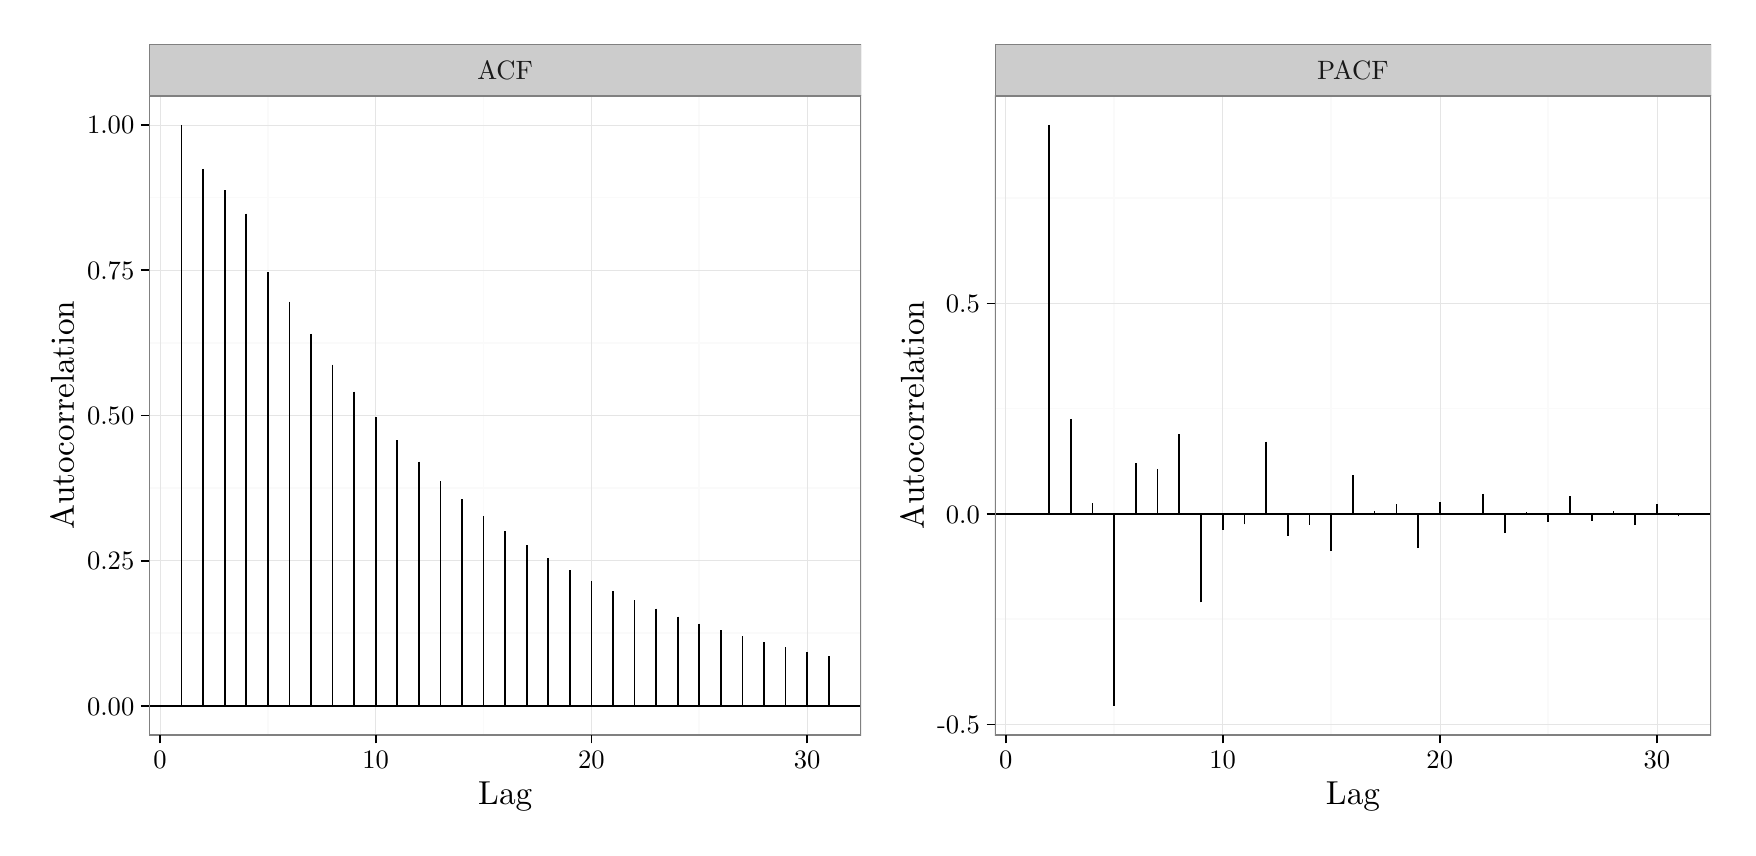
\begin{tikzpicture}[x=1pt,y=1pt]
\definecolor{fillColor}{RGB}{255,255,255}
\path[use as bounding box,fill=fillColor,fill opacity=0.00] (0,0) rectangle (614.29,289.08);
\begin{scope}
\path[clip] (  0.00,  0.00) rectangle (307.15,289.08);
\definecolor{drawColor}{RGB}{255,255,255}
\definecolor{fillColor}{RGB}{255,255,255}

\path[draw=drawColor,line width= 0.6pt,line join=round,line cap=round,fill=fillColor] ( -0.00,  0.00) rectangle (307.15,289.08);
\end{scope}
\begin{scope}
\path[clip] ( 43.93, 33.48) rectangle (301.15,264.47);
\definecolor{fillColor}{RGB}{255,255,255}

\path[fill=fillColor] ( 43.93, 33.48) rectangle (301.15,264.47);
\definecolor{drawColor}{gray}{0.98}

\path[draw=drawColor,line width= 0.6pt,line join=round] ( 43.93, 70.23) --
	(301.15, 70.23);

\path[draw=drawColor,line width= 0.6pt,line join=round] ( 43.93,122.72) --
	(301.15,122.72);

\path[draw=drawColor,line width= 0.6pt,line join=round] ( 43.93,175.22) --
	(301.15,175.22);

\path[draw=drawColor,line width= 0.6pt,line join=round] ( 43.93,227.72) --
	(301.15,227.72);

\path[draw=drawColor,line width= 0.6pt,line join=round] ( 86.80, 33.48) --
	( 86.80,264.47);

\path[draw=drawColor,line width= 0.6pt,line join=round] (164.74, 33.48) --
	(164.74,264.47);

\path[draw=drawColor,line width= 0.6pt,line join=round] (242.69, 33.48) --
	(242.69,264.47);
\definecolor{drawColor}{gray}{0.90}

\path[draw=drawColor,line width= 0.2pt,line join=round] ( 43.93, 43.98) --
	(301.15, 43.98);

\path[draw=drawColor,line width= 0.2pt,line join=round] ( 43.93, 96.47) --
	(301.15, 96.47);

\path[draw=drawColor,line width= 0.2pt,line join=round] ( 43.93,148.97) --
	(301.15,148.97);

\path[draw=drawColor,line width= 0.2pt,line join=round] ( 43.93,201.47) --
	(301.15,201.47);

\path[draw=drawColor,line width= 0.2pt,line join=round] ( 43.93,253.97) --
	(301.15,253.97);

\path[draw=drawColor,line width= 0.2pt,line join=round] ( 47.82, 33.48) --
	( 47.82,264.47);

\path[draw=drawColor,line width= 0.2pt,line join=round] (125.77, 33.48) --
	(125.77,264.47);

\path[draw=drawColor,line width= 0.2pt,line join=round] (203.72, 33.48) --
	(203.72,264.47);

\path[draw=drawColor,line width= 0.2pt,line join=round] (281.66, 33.48) --
	(281.66,264.47);
\definecolor{drawColor}{RGB}{0,0,0}

\path[draw=drawColor,line width= 0.6pt,line join=round] ( 43.93, 43.98) -- (301.15, 43.98);

\path[draw=drawColor,line width= 0.6pt,line join=round] ( 55.62,253.97) -- ( 55.62, 43.98);

\path[draw=drawColor,line width= 0.6pt,line join=round] ( 63.41,238.08) -- ( 63.41, 43.98);

\path[draw=drawColor,line width= 0.6pt,line join=round] ( 71.21,230.30) -- ( 71.21, 43.98);

\path[draw=drawColor,line width= 0.6pt,line join=round] ( 79.00,221.87) -- ( 79.00, 43.98);

\path[draw=drawColor,line width= 0.6pt,line join=round] ( 86.80,200.64) -- ( 86.80, 43.98);

\path[draw=drawColor,line width= 0.6pt,line join=round] ( 94.59,190.07) -- ( 94.59, 43.98);

\path[draw=drawColor,line width= 0.6pt,line join=round] (102.39,178.43) -- (102.39, 43.98);

\path[draw=drawColor,line width= 0.6pt,line join=round] (110.18,167.31) -- (110.18, 43.98);

\path[draw=drawColor,line width= 0.6pt,line join=round] (117.98,157.52) -- (117.98, 43.98);

\path[draw=drawColor,line width= 0.6pt,line join=round] (125.77,148.39) -- (125.77, 43.98);

\path[draw=drawColor,line width= 0.6pt,line join=round] (133.56,139.98) -- (133.56, 43.98);

\path[draw=drawColor,line width= 0.6pt,line join=round] (141.36,132.27) -- (141.36, 43.98);

\path[draw=drawColor,line width= 0.6pt,line join=round] (149.15,125.18) -- (149.15, 43.98);

\path[draw=drawColor,line width= 0.6pt,line join=round] (156.95,118.65) -- (156.95, 43.98);

\path[draw=drawColor,line width= 0.6pt,line join=round] (164.74,112.65) -- (164.74, 43.98);

\path[draw=drawColor,line width= 0.6pt,line join=round] (172.54,107.13) -- (172.54, 43.98);

\path[draw=drawColor,line width= 0.6pt,line join=round] (180.33,102.06) -- (180.33, 43.98);

\path[draw=drawColor,line width= 0.6pt,line join=round] (188.13, 97.39) -- (188.13, 43.98);

\path[draw=drawColor,line width= 0.6pt,line join=round] (195.92, 93.10) -- (195.92, 43.98);

\path[draw=drawColor,line width= 0.6pt,line join=round] (203.72, 89.15) -- (203.72, 43.98);

\path[draw=drawColor,line width= 0.6pt,line join=round] (211.51, 85.52) -- (211.51, 43.98);

\path[draw=drawColor,line width= 0.6pt,line join=round] (219.30, 82.18) -- (219.30, 43.98);

\path[draw=drawColor,line width= 0.6pt,line join=round] (227.10, 79.11) -- (227.10, 43.98);

\path[draw=drawColor,line width= 0.6pt,line join=round] (234.89, 76.29) -- (234.89, 43.98);

\path[draw=drawColor,line width= 0.6pt,line join=round] (242.69, 73.69) -- (242.69, 43.98);

\path[draw=drawColor,line width= 0.6pt,line join=round] (250.48, 71.30) -- (250.48, 43.98);

\path[draw=drawColor,line width= 0.6pt,line join=round] (258.28, 69.11) -- (258.28, 43.98);

\path[draw=drawColor,line width= 0.6pt,line join=round] (266.07, 67.09) -- (266.07, 43.98);

\path[draw=drawColor,line width= 0.6pt,line join=round] (273.87, 65.23) -- (273.87, 43.98);

\path[draw=drawColor,line width= 0.6pt,line join=round] (281.66, 63.52) -- (281.66, 43.98);

\path[draw=drawColor,line width= 0.6pt,line join=round] (289.46, 61.95) -- (289.46, 43.98);
\definecolor{drawColor}{gray}{0.50}

\path[draw=drawColor,line width= 0.6pt,line join=round,line cap=round] ( 43.93, 33.48) rectangle (301.15,264.47);
\end{scope}
\begin{scope}
\path[clip] ( 43.93,264.47) rectangle (301.15,283.08);
\definecolor{drawColor}{gray}{0.50}
\definecolor{fillColor}{gray}{0.80}

\path[draw=drawColor,line width= 0.2pt,line join=round,line cap=round,fill=fillColor] ( 43.93,264.47) rectangle (301.15,283.08);
\definecolor{drawColor}{gray}{0.10}

\node[text=drawColor,anchor=base,inner sep=0pt, outer sep=0pt, scale=  0.96] at (172.54,270.47) {ACF};
\end{scope}
\begin{scope}
\path[clip] (  0.00,  0.00) rectangle (614.29,289.08);
\definecolor{drawColor}{RGB}{0,0,0}

\node[text=drawColor,anchor=base east,inner sep=0pt, outer sep=0pt, scale=  0.96] at ( 38.53, 40.67) {0.00};

\node[text=drawColor,anchor=base east,inner sep=0pt, outer sep=0pt, scale=  0.96] at ( 38.53, 93.17) {0.25};

\node[text=drawColor,anchor=base east,inner sep=0pt, outer sep=0pt, scale=  0.96] at ( 38.53,145.67) {0.50};

\node[text=drawColor,anchor=base east,inner sep=0pt, outer sep=0pt, scale=  0.96] at ( 38.53,198.16) {0.75};

\node[text=drawColor,anchor=base east,inner sep=0pt, outer sep=0pt, scale=  0.96] at ( 38.53,250.66) {1.00};
\end{scope}
\begin{scope}
\path[clip] (  0.00,  0.00) rectangle (614.29,289.08);
\definecolor{drawColor}{RGB}{0,0,0}

\path[draw=drawColor,line width= 0.6pt,line join=round] ( 40.93, 43.98) --
	( 43.93, 43.98);

\path[draw=drawColor,line width= 0.6pt,line join=round] ( 40.93, 96.47) --
	( 43.93, 96.47);

\path[draw=drawColor,line width= 0.6pt,line join=round] ( 40.93,148.97) --
	( 43.93,148.97);

\path[draw=drawColor,line width= 0.6pt,line join=round] ( 40.93,201.47) --
	( 43.93,201.47);

\path[draw=drawColor,line width= 0.6pt,line join=round] ( 40.93,253.97) --
	( 43.93,253.97);
\end{scope}
\begin{scope}
\path[clip] (  0.00,  0.00) rectangle (614.29,289.08);
\definecolor{drawColor}{RGB}{0,0,0}

\path[draw=drawColor,line width= 0.6pt,line join=round] ( 47.82, 30.48) --
	( 47.82, 33.48);

\path[draw=drawColor,line width= 0.6pt,line join=round] (125.77, 30.48) --
	(125.77, 33.48);

\path[draw=drawColor,line width= 0.6pt,line join=round] (203.72, 30.48) --
	(203.72, 33.48);

\path[draw=drawColor,line width= 0.6pt,line join=round] (281.66, 30.48) --
	(281.66, 33.48);
\end{scope}
\begin{scope}
\path[clip] (  0.00,  0.00) rectangle (614.29,289.08);
\definecolor{drawColor}{RGB}{0,0,0}

\node[text=drawColor,anchor=base,inner sep=0pt, outer sep=0pt, scale=  0.96] at ( 47.82, 21.46) {0};

\node[text=drawColor,anchor=base,inner sep=0pt, outer sep=0pt, scale=  0.96] at (125.77, 21.46) {10};

\node[text=drawColor,anchor=base,inner sep=0pt, outer sep=0pt, scale=  0.96] at (203.72, 21.46) {20};

\node[text=drawColor,anchor=base,inner sep=0pt, outer sep=0pt, scale=  0.96] at (281.66, 21.46) {30};
\end{scope}
\begin{scope}
\path[clip] (  0.00,  0.00) rectangle (614.29,289.08);
\definecolor{drawColor}{RGB}{0,0,0}

\node[text=drawColor,anchor=base,inner sep=0pt, outer sep=0pt, scale=  1.20] at (172.54,  8.40) {Lag};
\end{scope}
\begin{scope}
\path[clip] (  0.00,  0.00) rectangle (614.29,289.08);
\definecolor{drawColor}{RGB}{0,0,0}

\node[text=drawColor,rotate= 90.00,anchor=base,inner sep=0pt, outer sep=0pt, scale=  1.20] at ( 16.66,148.97) {Autocorrelation};
\end{scope}
\begin{scope}
\path[clip] (307.15,  0.00) rectangle (614.29,289.08);
\definecolor{drawColor}{RGB}{255,255,255}
\definecolor{fillColor}{RGB}{255,255,255}

\path[draw=drawColor,line width= 0.6pt,line join=round,line cap=round,fill=fillColor] (307.15,  0.00) rectangle (614.29,289.08);
\end{scope}
\begin{scope}
\path[clip] (349.48, 33.48) rectangle (608.30,264.47);
\definecolor{fillColor}{RGB}{255,255,255}

\path[fill=fillColor] (349.48, 33.48) rectangle (608.29,264.47);
\definecolor{drawColor}{gray}{0.98}

\path[draw=drawColor,line width= 0.6pt,line join=round] (349.48, 75.36) --
	(608.30, 75.36);

\path[draw=drawColor,line width= 0.6pt,line join=round] (349.48,151.41) --
	(608.30,151.41);

\path[draw=drawColor,line width= 0.6pt,line join=round] (349.48,227.45) --
	(608.30,227.45);

\path[draw=drawColor,line width= 0.6pt,line join=round] (392.61, 33.48) --
	(392.61,264.47);

\path[draw=drawColor,line width= 0.6pt,line join=round] (471.04, 33.48) --
	(471.04,264.47);

\path[draw=drawColor,line width= 0.6pt,line join=round] (549.47, 33.48) --
	(549.47,264.47);
\definecolor{drawColor}{gray}{0.90}

\path[draw=drawColor,line width= 0.2pt,line join=round] (349.48, 37.34) --
	(608.30, 37.34);

\path[draw=drawColor,line width= 0.2pt,line join=round] (349.48,113.39) --
	(608.30,113.39);

\path[draw=drawColor,line width= 0.2pt,line join=round] (349.48,189.43) --
	(608.30,189.43);

\path[draw=drawColor,line width= 0.2pt,line join=round] (353.40, 33.48) --
	(353.40,264.47);

\path[draw=drawColor,line width= 0.2pt,line join=round] (431.83, 33.48) --
	(431.83,264.47);

\path[draw=drawColor,line width= 0.2pt,line join=round] (510.26, 33.48) --
	(510.26,264.47);

\path[draw=drawColor,line width= 0.2pt,line join=round] (588.69, 33.48) --
	(588.69,264.47);
\definecolor{drawColor}{RGB}{0,0,0}

\path[draw=drawColor,line width= 0.6pt,line join=round] (349.48,113.39) -- (608.30,113.39);

\path[draw=drawColor,line width= 0.6pt,line join=round] (369.08,253.97) -- (369.08,113.39);

\path[draw=drawColor,line width= 0.6pt,line join=round] (376.93,147.73) -- (376.93,113.39);

\path[draw=drawColor,line width= 0.6pt,line join=round] (384.77,117.17) -- (384.77,113.39);

\path[draw=drawColor,line width= 0.6pt,line join=round] (392.61, 43.98) -- (392.61,113.39);

\path[draw=drawColor,line width= 0.6pt,line join=round] (400.45,131.74) -- (400.45,113.39);

\path[draw=drawColor,line width= 0.6pt,line join=round] (408.30,129.65) -- (408.30,113.39);

\path[draw=drawColor,line width= 0.6pt,line join=round] (416.14,142.23) -- (416.14,113.39);

\path[draw=drawColor,line width= 0.6pt,line join=round] (423.98, 81.41) -- (423.98,113.39);

\path[draw=drawColor,line width= 0.6pt,line join=round] (431.83,107.60) -- (431.83,113.39);

\path[draw=drawColor,line width= 0.6pt,line join=round] (439.67,109.61) -- (439.67,113.39);

\path[draw=drawColor,line width= 0.6pt,line join=round] (447.51,139.51) -- (447.51,113.39);

\path[draw=drawColor,line width= 0.6pt,line join=round] (455.36,105.57) -- (455.36,113.39);

\path[draw=drawColor,line width= 0.6pt,line join=round] (463.20,109.49) -- (463.20,113.39);

\path[draw=drawColor,line width= 0.6pt,line join=round] (471.04, 99.91) -- (471.04,113.39);

\path[draw=drawColor,line width= 0.6pt,line join=round] (478.89,127.41) -- (478.89,113.39);

\path[draw=drawColor,line width= 0.6pt,line join=round] (486.73,114.39) -- (486.73,113.39);

\path[draw=drawColor,line width= 0.6pt,line join=round] (494.57,116.95) -- (494.57,113.39);

\path[draw=drawColor,line width= 0.6pt,line join=round] (502.41,101.00) -- (502.41,113.39);

\path[draw=drawColor,line width= 0.6pt,line join=round] (510.26,117.63) -- (510.26,113.39);

\path[draw=drawColor,line width= 0.6pt,line join=round] (518.10,113.58) -- (518.10,113.39);

\path[draw=drawColor,line width= 0.6pt,line join=round] (525.94,120.62) -- (525.94,113.39);

\path[draw=drawColor,line width= 0.6pt,line join=round] (533.79,106.46) -- (533.79,113.39);

\path[draw=drawColor,line width= 0.6pt,line join=round] (541.63,113.94) -- (541.63,113.39);

\path[draw=drawColor,line width= 0.6pt,line join=round] (549.47,110.58) -- (549.47,113.39);

\path[draw=drawColor,line width= 0.6pt,line join=round] (557.32,119.70) -- (557.32,113.39);

\path[draw=drawColor,line width= 0.6pt,line join=round] (565.16,110.82) -- (565.16,113.39);

\path[draw=drawColor,line width= 0.6pt,line join=round] (573.00,114.26) -- (573.00,113.39);

\path[draw=drawColor,line width= 0.6pt,line join=round] (580.84,109.33) -- (580.84,113.39);

\path[draw=drawColor,line width= 0.6pt,line join=round] (588.69,117.04) -- (588.69,113.39);

\path[draw=drawColor,line width= 0.6pt,line join=round] (596.53,112.47) -- (596.53,113.39);
\definecolor{drawColor}{gray}{0.50}

\path[draw=drawColor,line width= 0.6pt,line join=round,line cap=round] (349.48, 33.48) rectangle (608.29,264.47);
\end{scope}
\begin{scope}
\path[clip] (349.48,264.47) rectangle (608.30,283.08);
\definecolor{drawColor}{gray}{0.50}
\definecolor{fillColor}{gray}{0.80}

\path[draw=drawColor,line width= 0.2pt,line join=round,line cap=round,fill=fillColor] (349.48,264.47) rectangle (608.29,283.08);
\definecolor{drawColor}{gray}{0.10}

\node[text=drawColor,anchor=base,inner sep=0pt, outer sep=0pt, scale=  0.96] at (478.89,270.47) {PACF};
\end{scope}
\begin{scope}
\path[clip] (  0.00,  0.00) rectangle (614.29,289.08);
\definecolor{drawColor}{RGB}{0,0,0}

\node[text=drawColor,anchor=base east,inner sep=0pt, outer sep=0pt, scale=  0.96] at (344.08, 34.04) {-0.5};

\node[text=drawColor,anchor=base east,inner sep=0pt, outer sep=0pt, scale=  0.96] at (344.08,110.08) {0.0};

\node[text=drawColor,anchor=base east,inner sep=0pt, outer sep=0pt, scale=  0.96] at (344.08,186.12) {0.5};
\end{scope}
\begin{scope}
\path[clip] (  0.00,  0.00) rectangle (614.29,289.08);
\definecolor{drawColor}{RGB}{0,0,0}

\path[draw=drawColor,line width= 0.6pt,line join=round] (346.48, 37.34) --
	(349.48, 37.34);

\path[draw=drawColor,line width= 0.6pt,line join=round] (346.48,113.39) --
	(349.48,113.39);

\path[draw=drawColor,line width= 0.6pt,line join=round] (346.48,189.43) --
	(349.48,189.43);
\end{scope}
\begin{scope}
\path[clip] (  0.00,  0.00) rectangle (614.29,289.08);
\definecolor{drawColor}{RGB}{0,0,0}

\path[draw=drawColor,line width= 0.6pt,line join=round] (353.40, 30.48) --
	(353.40, 33.48);

\path[draw=drawColor,line width= 0.6pt,line join=round] (431.83, 30.48) --
	(431.83, 33.48);

\path[draw=drawColor,line width= 0.6pt,line join=round] (510.26, 30.48) --
	(510.26, 33.48);

\path[draw=drawColor,line width= 0.6pt,line join=round] (588.69, 30.48) --
	(588.69, 33.48);
\end{scope}
\begin{scope}
\path[clip] (  0.00,  0.00) rectangle (614.29,289.08);
\definecolor{drawColor}{RGB}{0,0,0}

\node[text=drawColor,anchor=base,inner sep=0pt, outer sep=0pt, scale=  0.96] at (353.40, 21.46) {0};

\node[text=drawColor,anchor=base,inner sep=0pt, outer sep=0pt, scale=  0.96] at (431.83, 21.46) {10};

\node[text=drawColor,anchor=base,inner sep=0pt, outer sep=0pt, scale=  0.96] at (510.26, 21.46) {20};

\node[text=drawColor,anchor=base,inner sep=0pt, outer sep=0pt, scale=  0.96] at (588.69, 21.46) {30};
\end{scope}
\begin{scope}
\path[clip] (  0.00,  0.00) rectangle (614.29,289.08);
\definecolor{drawColor}{RGB}{0,0,0}

\node[text=drawColor,anchor=base,inner sep=0pt, outer sep=0pt, scale=  1.20] at (478.89,  8.40) {Lag};
\end{scope}
\begin{scope}
\path[clip] (  0.00,  0.00) rectangle (614.29,289.08);
\definecolor{drawColor}{RGB}{0,0,0}

\node[text=drawColor,rotate= 90.00,anchor=base,inner sep=0pt, outer sep=0pt, scale=  1.20] at (323.81,148.97) {Autocorrelation};
\end{scope}
\end{tikzpicture}
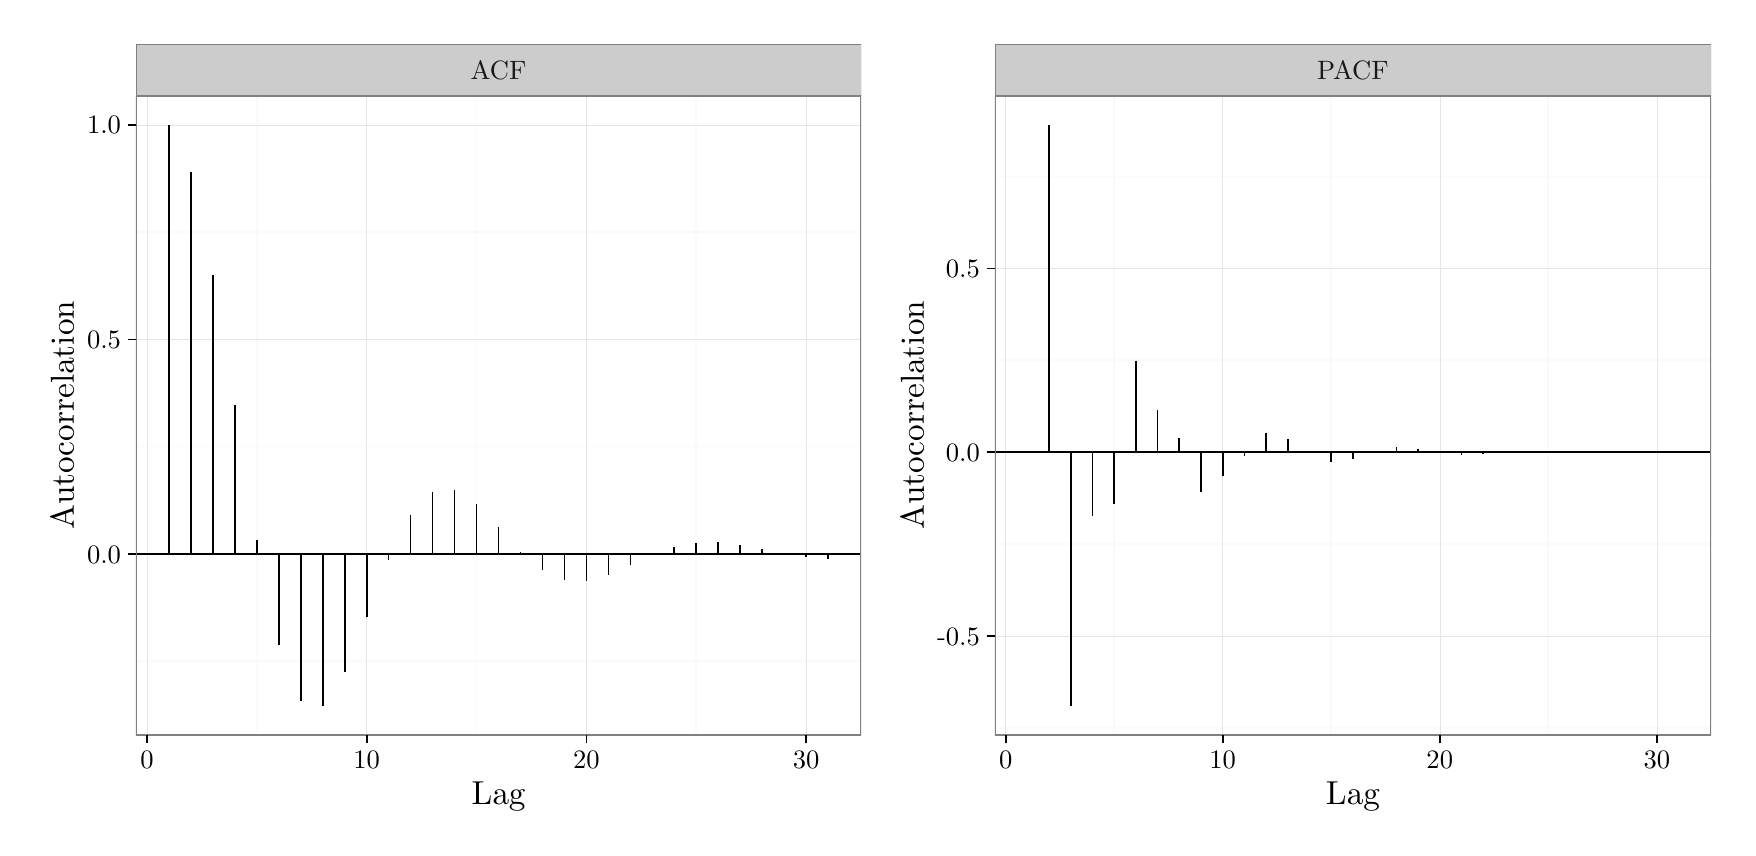
\begin{tikzpicture}[x=1pt,y=1pt]
\definecolor{fillColor}{RGB}{255,255,255}
\path[use as bounding box,fill=fillColor,fill opacity=0.00] (0,0) rectangle (614.29,289.08);
\begin{scope}
\path[clip] (  0.00,  0.00) rectangle (307.15,289.08);
\definecolor{drawColor}{RGB}{255,255,255}
\definecolor{fillColor}{RGB}{255,255,255}

\path[draw=drawColor,line width= 0.6pt,line join=round,line cap=round,fill=fillColor] (  0.00,  0.00) rectangle (307.15,289.08);
\end{scope}
\begin{scope}
\path[clip] ( 39.13, 33.48) rectangle (301.15,264.47);
\definecolor{fillColor}{RGB}{255,255,255}

\path[fill=fillColor] ( 39.13, 33.48) rectangle (301.15,264.47);
\definecolor{drawColor}{gray}{0.98}

\path[draw=drawColor,line width= 0.6pt,line join=round] ( 39.13, 60.16) --
	(301.15, 60.16);

\path[draw=drawColor,line width= 0.6pt,line join=round] ( 39.13,137.68) --
	(301.15,137.68);

\path[draw=drawColor,line width= 0.6pt,line join=round] ( 39.13,215.21) --
	(301.15,215.21);

\path[draw=drawColor,line width= 0.6pt,line join=round] ( 82.80, 33.48) --
	( 82.80,264.47);

\path[draw=drawColor,line width= 0.6pt,line join=round] (162.20, 33.48) --
	(162.20,264.47);

\path[draw=drawColor,line width= 0.6pt,line join=round] (241.60, 33.48) --
	(241.60,264.47);
\definecolor{drawColor}{gray}{0.90}

\path[draw=drawColor,line width= 0.2pt,line join=round] ( 39.13, 98.92) --
	(301.15, 98.92);

\path[draw=drawColor,line width= 0.2pt,line join=round] ( 39.13,176.45) --
	(301.15,176.45);

\path[draw=drawColor,line width= 0.2pt,line join=round] ( 39.13,253.97) --
	(301.15,253.97);

\path[draw=drawColor,line width= 0.2pt,line join=round] ( 43.10, 33.48) --
	( 43.10,264.47);

\path[draw=drawColor,line width= 0.2pt,line join=round] (122.50, 33.48) --
	(122.50,264.47);

\path[draw=drawColor,line width= 0.2pt,line join=round] (201.90, 33.48) --
	(201.90,264.47);

\path[draw=drawColor,line width= 0.2pt,line join=round] (281.30, 33.48) --
	(281.30,264.47);
\definecolor{drawColor}{RGB}{0,0,0}

\path[draw=drawColor,line width= 0.6pt,line join=round] ( 39.13, 98.92) -- (301.15, 98.92);

\path[draw=drawColor,line width= 0.6pt,line join=round] ( 51.04,253.97) -- ( 51.04, 98.92);

\path[draw=drawColor,line width= 0.6pt,line join=round] ( 58.98,237.04) -- ( 58.98, 98.92);

\path[draw=drawColor,line width= 0.6pt,line join=round] ( 66.92,199.85) -- ( 66.92, 98.92);

\path[draw=drawColor,line width= 0.6pt,line join=round] ( 74.86,152.64) -- ( 74.86, 98.92);

\path[draw=drawColor,line width= 0.6pt,line join=round] ( 82.80,103.79) -- ( 82.80, 98.92);

\path[draw=drawColor,line width= 0.6pt,line join=round] ( 90.74, 65.94) -- ( 90.74, 98.92);

\path[draw=drawColor,line width= 0.6pt,line join=round] ( 98.68, 45.80) -- ( 98.68, 98.92);

\path[draw=drawColor,line width= 0.6pt,line join=round] (106.62, 43.98) -- (106.62, 98.92);

\path[draw=drawColor,line width= 0.6pt,line join=round] (114.56, 56.34) -- (114.56, 98.92);

\path[draw=drawColor,line width= 0.6pt,line join=round] (122.50, 76.26) -- (122.50, 98.92);

\path[draw=drawColor,line width= 0.6pt,line join=round] (130.44, 96.87) -- (130.44, 98.92);

\path[draw=drawColor,line width= 0.6pt,line join=round] (138.38,112.84) -- (138.38, 98.92);

\path[draw=drawColor,line width= 0.6pt,line join=round] (146.32,121.33) -- (146.32, 98.92);

\path[draw=drawColor,line width= 0.6pt,line join=round] (154.26,122.10) -- (154.26, 98.92);

\path[draw=drawColor,line width= 0.6pt,line join=round] (162.20,116.89) -- (162.20, 98.92);

\path[draw=drawColor,line width= 0.6pt,line join=round] (170.14,108.48) -- (170.14, 98.92);

\path[draw=drawColor,line width= 0.6pt,line join=round] (178.08, 99.79) -- (178.08, 98.92);

\path[draw=drawColor,line width= 0.6pt,line join=round] (186.02, 93.05) -- (186.02, 98.92);

\path[draw=drawColor,line width= 0.6pt,line join=round] (193.96, 89.47) -- (193.96, 98.92);

\path[draw=drawColor,line width= 0.6pt,line join=round] (201.90, 89.14) -- (201.90, 98.92);

\path[draw=drawColor,line width= 0.6pt,line join=round] (209.84, 91.34) -- (209.84, 98.92);

\path[draw=drawColor,line width= 0.6pt,line join=round] (217.78, 94.89) -- (217.78, 98.92);

\path[draw=drawColor,line width= 0.6pt,line join=round] (225.72, 98.56) -- (225.72, 98.92);

\path[draw=drawColor,line width= 0.6pt,line join=round] (233.66,101.40) -- (233.66, 98.92);

\path[draw=drawColor,line width= 0.6pt,line join=round] (241.60,102.91) -- (241.60, 98.92);

\path[draw=drawColor,line width= 0.6pt,line join=round] (249.54,103.05) -- (249.54, 98.92);

\path[draw=drawColor,line width= 0.6pt,line join=round] (257.48,102.12) -- (257.48, 98.92);

\path[draw=drawColor,line width= 0.6pt,line join=round] (265.42,100.62) -- (265.42, 98.92);

\path[draw=drawColor,line width= 0.6pt,line join=round] (273.36, 99.08) -- (273.36, 98.92);

\path[draw=drawColor,line width= 0.6pt,line join=round] (281.30, 97.88) -- (281.30, 98.92);

\path[draw=drawColor,line width= 0.6pt,line join=round] (289.24, 97.24) -- (289.24, 98.92);
\definecolor{drawColor}{gray}{0.50}

\path[draw=drawColor,line width= 0.6pt,line join=round,line cap=round] ( 39.13, 33.48) rectangle (301.15,264.47);
\end{scope}
\begin{scope}
\path[clip] ( 39.13,264.47) rectangle (301.15,283.08);
\definecolor{drawColor}{gray}{0.50}
\definecolor{fillColor}{gray}{0.80}

\path[draw=drawColor,line width= 0.2pt,line join=round,line cap=round,fill=fillColor] ( 39.13,264.47) rectangle (301.15,283.08);
\definecolor{drawColor}{gray}{0.10}

\node[text=drawColor,anchor=base,inner sep=0pt, outer sep=0pt, scale=  0.96] at (170.14,270.47) {ACF};
\end{scope}
\begin{scope}
\path[clip] (  0.00,  0.00) rectangle (614.29,289.08);
\definecolor{drawColor}{RGB}{0,0,0}

\node[text=drawColor,anchor=base east,inner sep=0pt, outer sep=0pt, scale=  0.96] at ( 33.73, 95.62) {0.0};

\node[text=drawColor,anchor=base east,inner sep=0pt, outer sep=0pt, scale=  0.96] at ( 33.73,173.14) {0.5};

\node[text=drawColor,anchor=base east,inner sep=0pt, outer sep=0pt, scale=  0.96] at ( 33.73,250.66) {1.0};
\end{scope}
\begin{scope}
\path[clip] (  0.00,  0.00) rectangle (614.29,289.08);
\definecolor{drawColor}{RGB}{0,0,0}

\path[draw=drawColor,line width= 0.6pt,line join=round] ( 36.13, 98.92) --
	( 39.13, 98.92);

\path[draw=drawColor,line width= 0.6pt,line join=round] ( 36.13,176.45) --
	( 39.13,176.45);

\path[draw=drawColor,line width= 0.6pt,line join=round] ( 36.13,253.97) --
	( 39.13,253.97);
\end{scope}
\begin{scope}
\path[clip] (  0.00,  0.00) rectangle (614.29,289.08);
\definecolor{drawColor}{RGB}{0,0,0}

\path[draw=drawColor,line width= 0.6pt,line join=round] ( 43.10, 30.48) --
	( 43.10, 33.48);

\path[draw=drawColor,line width= 0.6pt,line join=round] (122.50, 30.48) --
	(122.50, 33.48);

\path[draw=drawColor,line width= 0.6pt,line join=round] (201.90, 30.48) --
	(201.90, 33.48);

\path[draw=drawColor,line width= 0.6pt,line join=round] (281.30, 30.48) --
	(281.30, 33.48);
\end{scope}
\begin{scope}
\path[clip] (  0.00,  0.00) rectangle (614.29,289.08);
\definecolor{drawColor}{RGB}{0,0,0}

\node[text=drawColor,anchor=base,inner sep=0pt, outer sep=0pt, scale=  0.96] at ( 43.10, 21.46) {0};

\node[text=drawColor,anchor=base,inner sep=0pt, outer sep=0pt, scale=  0.96] at (122.50, 21.46) {10};

\node[text=drawColor,anchor=base,inner sep=0pt, outer sep=0pt, scale=  0.96] at (201.90, 21.46) {20};

\node[text=drawColor,anchor=base,inner sep=0pt, outer sep=0pt, scale=  0.96] at (281.30, 21.46) {30};
\end{scope}
\begin{scope}
\path[clip] (  0.00,  0.00) rectangle (614.29,289.08);
\definecolor{drawColor}{RGB}{0,0,0}

\node[text=drawColor,anchor=base,inner sep=0pt, outer sep=0pt, scale=  1.20] at (170.14,  8.40) {Lag};
\end{scope}
\begin{scope}
\path[clip] (  0.00,  0.00) rectangle (614.29,289.08);
\definecolor{drawColor}{RGB}{0,0,0}

\node[text=drawColor,rotate= 90.00,anchor=base,inner sep=0pt, outer sep=0pt, scale=  1.20] at ( 16.66,148.97) {Autocorrelation};
\end{scope}
\begin{scope}
\path[clip] (307.15,  0.00) rectangle (614.29,289.08);
\definecolor{drawColor}{RGB}{255,255,255}
\definecolor{fillColor}{RGB}{255,255,255}

\path[draw=drawColor,line width= 0.6pt,line join=round,line cap=round,fill=fillColor] (307.15,  0.00) rectangle (614.29,289.08);
\end{scope}
\begin{scope}
\path[clip] (349.48, 33.48) rectangle (608.30,264.47);
\definecolor{fillColor}{RGB}{255,255,255}

\path[fill=fillColor] (349.48, 33.48) rectangle (608.29,264.47);
\definecolor{drawColor}{gray}{0.98}

\path[draw=drawColor,line width= 0.6pt,line join=round] (349.48, 36.10) --
	(608.30, 36.10);

\path[draw=drawColor,line width= 0.6pt,line join=round] (349.48,102.49) --
	(608.30,102.49);

\path[draw=drawColor,line width= 0.6pt,line join=round] (349.48,168.88) --
	(608.30,168.88);

\path[draw=drawColor,line width= 0.6pt,line join=round] (349.48,235.27) --
	(608.30,235.27);

\path[draw=drawColor,line width= 0.6pt,line join=round] (392.61, 33.48) --
	(392.61,264.47);

\path[draw=drawColor,line width= 0.6pt,line join=round] (471.04, 33.48) --
	(471.04,264.47);

\path[draw=drawColor,line width= 0.6pt,line join=round] (549.47, 33.48) --
	(549.47,264.47);
\definecolor{drawColor}{gray}{0.90}

\path[draw=drawColor,line width= 0.2pt,line join=round] (349.48, 69.30) --
	(608.30, 69.30);

\path[draw=drawColor,line width= 0.2pt,line join=round] (349.48,135.69) --
	(608.30,135.69);

\path[draw=drawColor,line width= 0.2pt,line join=round] (349.48,202.08) --
	(608.30,202.08);

\path[draw=drawColor,line width= 0.2pt,line join=round] (353.40, 33.48) --
	(353.40,264.47);

\path[draw=drawColor,line width= 0.2pt,line join=round] (431.83, 33.48) --
	(431.83,264.47);

\path[draw=drawColor,line width= 0.2pt,line join=round] (510.26, 33.48) --
	(510.26,264.47);

\path[draw=drawColor,line width= 0.2pt,line join=round] (588.69, 33.48) --
	(588.69,264.47);
\definecolor{drawColor}{RGB}{0,0,0}

\path[draw=drawColor,line width= 0.6pt,line join=round] (349.48,135.69) -- (608.30,135.69);

\path[draw=drawColor,line width= 0.6pt,line join=round] (369.08,253.97) -- (369.08,135.69);

\path[draw=drawColor,line width= 0.6pt,line join=round] (376.93, 43.98) -- (376.93,135.69);

\path[draw=drawColor,line width= 0.6pt,line join=round] (384.77,112.67) -- (384.77,135.69);

\path[draw=drawColor,line width= 0.6pt,line join=round] (392.61,116.96) -- (392.61,135.69);

\path[draw=drawColor,line width= 0.6pt,line join=round] (400.45,168.74) -- (400.45,135.69);

\path[draw=drawColor,line width= 0.6pt,line join=round] (408.30,150.75) -- (408.30,135.69);

\path[draw=drawColor,line width= 0.6pt,line join=round] (416.14,140.72) -- (416.14,135.69);

\path[draw=drawColor,line width= 0.6pt,line join=round] (423.98,121.27) -- (423.98,135.69);

\path[draw=drawColor,line width= 0.6pt,line join=round] (431.83,126.98) -- (431.83,135.69);

\path[draw=drawColor,line width= 0.6pt,line join=round] (439.67,134.40) -- (439.67,135.69);

\path[draw=drawColor,line width= 0.6pt,line join=round] (447.51,142.57) -- (447.51,135.69);

\path[draw=drawColor,line width= 0.6pt,line join=round] (455.36,140.38) -- (455.36,135.69);

\path[draw=drawColor,line width= 0.6pt,line join=round] (463.20,135.92) -- (463.20,135.69);

\path[draw=drawColor,line width= 0.6pt,line join=round] (471.04,132.25) -- (471.04,135.69);

\path[draw=drawColor,line width= 0.6pt,line join=round] (478.89,133.25) -- (478.89,135.69);

\path[draw=drawColor,line width= 0.6pt,line join=round] (486.73,135.73) -- (486.73,135.69);

\path[draw=drawColor,line width= 0.6pt,line join=round] (494.57,137.44) -- (494.57,135.69);

\path[draw=drawColor,line width= 0.6pt,line join=round] (502.41,136.93) -- (502.41,135.69);

\path[draw=drawColor,line width= 0.6pt,line join=round] (510.26,135.60) -- (510.26,135.69);

\path[draw=drawColor,line width= 0.6pt,line join=round] (518.10,134.78) -- (518.10,135.69);

\path[draw=drawColor,line width= 0.6pt,line join=round] (525.94,135.06) -- (525.94,135.69);

\path[draw=drawColor,line width= 0.6pt,line join=round] (533.79,135.76) -- (533.79,135.69);

\path[draw=drawColor,line width= 0.6pt,line join=round] (541.63,136.16) -- (541.63,135.69);

\path[draw=drawColor,line width= 0.6pt,line join=round] (549.47,136.00) -- (549.47,135.69);

\path[draw=drawColor,line width= 0.6pt,line join=round] (557.32,135.64) -- (557.32,135.69);

\path[draw=drawColor,line width= 0.6pt,line join=round] (565.16,135.44) -- (565.16,135.69);

\path[draw=drawColor,line width= 0.6pt,line join=round] (573.00,135.53) -- (573.00,135.69);

\path[draw=drawColor,line width= 0.6pt,line join=round] (580.84,135.72) -- (580.84,135.69);

\path[draw=drawColor,line width= 0.6pt,line join=round] (588.69,135.81) -- (588.69,135.69);

\path[draw=drawColor,line width= 0.6pt,line join=round] (596.53,135.76) -- (596.53,135.69);
\definecolor{drawColor}{gray}{0.50}

\path[draw=drawColor,line width= 0.6pt,line join=round,line cap=round] (349.48, 33.48) rectangle (608.29,264.47);
\end{scope}
\begin{scope}
\path[clip] (349.48,264.47) rectangle (608.30,283.08);
\definecolor{drawColor}{gray}{0.50}
\definecolor{fillColor}{gray}{0.80}

\path[draw=drawColor,line width= 0.2pt,line join=round,line cap=round,fill=fillColor] (349.48,264.47) rectangle (608.29,283.08);
\definecolor{drawColor}{gray}{0.10}

\node[text=drawColor,anchor=base,inner sep=0pt, outer sep=0pt, scale=  0.96] at (478.89,270.47) {PACF};
\end{scope}
\begin{scope}
\path[clip] (  0.00,  0.00) rectangle (614.29,289.08);
\definecolor{drawColor}{RGB}{0,0,0}

\node[text=drawColor,anchor=base east,inner sep=0pt, outer sep=0pt, scale=  0.96] at (344.08, 65.99) {-0.5};

\node[text=drawColor,anchor=base east,inner sep=0pt, outer sep=0pt, scale=  0.96] at (344.08,132.38) {0.0};

\node[text=drawColor,anchor=base east,inner sep=0pt, outer sep=0pt, scale=  0.96] at (344.08,198.77) {0.5};
\end{scope}
\begin{scope}
\path[clip] (  0.00,  0.00) rectangle (614.29,289.08);
\definecolor{drawColor}{RGB}{0,0,0}

\path[draw=drawColor,line width= 0.6pt,line join=round] (346.48, 69.30) --
	(349.48, 69.30);

\path[draw=drawColor,line width= 0.6pt,line join=round] (346.48,135.69) --
	(349.48,135.69);

\path[draw=drawColor,line width= 0.6pt,line join=round] (346.48,202.08) --
	(349.48,202.08);
\end{scope}
\begin{scope}
\path[clip] (  0.00,  0.00) rectangle (614.29,289.08);
\definecolor{drawColor}{RGB}{0,0,0}

\path[draw=drawColor,line width= 0.6pt,line join=round] (353.40, 30.48) --
	(353.40, 33.48);

\path[draw=drawColor,line width= 0.6pt,line join=round] (431.83, 30.48) --
	(431.83, 33.48);

\path[draw=drawColor,line width= 0.6pt,line join=round] (510.26, 30.48) --
	(510.26, 33.48);

\path[draw=drawColor,line width= 0.6pt,line join=round] (588.69, 30.48) --
	(588.69, 33.48);
\end{scope}
\begin{scope}
\path[clip] (  0.00,  0.00) rectangle (614.29,289.08);
\definecolor{drawColor}{RGB}{0,0,0}

\node[text=drawColor,anchor=base,inner sep=0pt, outer sep=0pt, scale=  0.96] at (353.40, 21.46) {0};

\node[text=drawColor,anchor=base,inner sep=0pt, outer sep=0pt, scale=  0.96] at (431.83, 21.46) {10};

\node[text=drawColor,anchor=base,inner sep=0pt, outer sep=0pt, scale=  0.96] at (510.26, 21.46) {20};

\node[text=drawColor,anchor=base,inner sep=0pt, outer sep=0pt, scale=  0.96] at (588.69, 21.46) {30};
\end{scope}
\begin{scope}
\path[clip] (  0.00,  0.00) rectangle (614.29,289.08);
\definecolor{drawColor}{RGB}{0,0,0}

\node[text=drawColor,anchor=base,inner sep=0pt, outer sep=0pt, scale=  1.20] at (478.89,  8.40) {Lag};
\end{scope}
\begin{scope}
\path[clip] (  0.00,  0.00) rectangle (614.29,289.08);
\definecolor{drawColor}{RGB}{0,0,0}

\node[text=drawColor,rotate= 90.00,anchor=base,inner sep=0pt, outer sep=0pt, scale=  1.20] at (323.81,148.97) {Autocorrelation};
\end{scope}
\end{tikzpicture}
